\documentclass{standalone}
\usepackage{tikz, bm}
\usetikzlibrary{bbox, angles, quotes, intersections}
\usetikzlibrary{calc}
\usetikzlibrary{arrows.meta,decorations.pathmorphing,backgrounds,positioning,fit,petri}

%\def\b{0.05}
\def\b{8}
\def\c{\b -1}
\def\ri{1}
\def\rri{2}
\def\rrri{3}
\def\rrrri{4}

\def\centerarc[#1](#2)(#3:#4:#5)% Syntax: [draw options] (center) (initial angle:final angle:radius)
    { \draw[#1] ($(#2)+({(#5)*cos(#3)},{(#5)*sin(#3)})$) arc (#3:#4:#5); }

\def\beamline[#1](#2)(#3:#4)% Syntax: [draw options] (radius) (initial angle:final angle:radius)
    {  \draw[#1] ({(#2-2*\b)*cos(#4)},-#3/2 * sin(#4)) -- ({(#2-2*\b)*cos(#4)},#3/2 * sin(#4)); 
    \draw ({(1-2*0.05)*cos(90)},{-1/2 * sin(90)}) -- ({(1-2*0.05)*cos(90)},{1/2 * sin(90)});
    }


\begin{document}

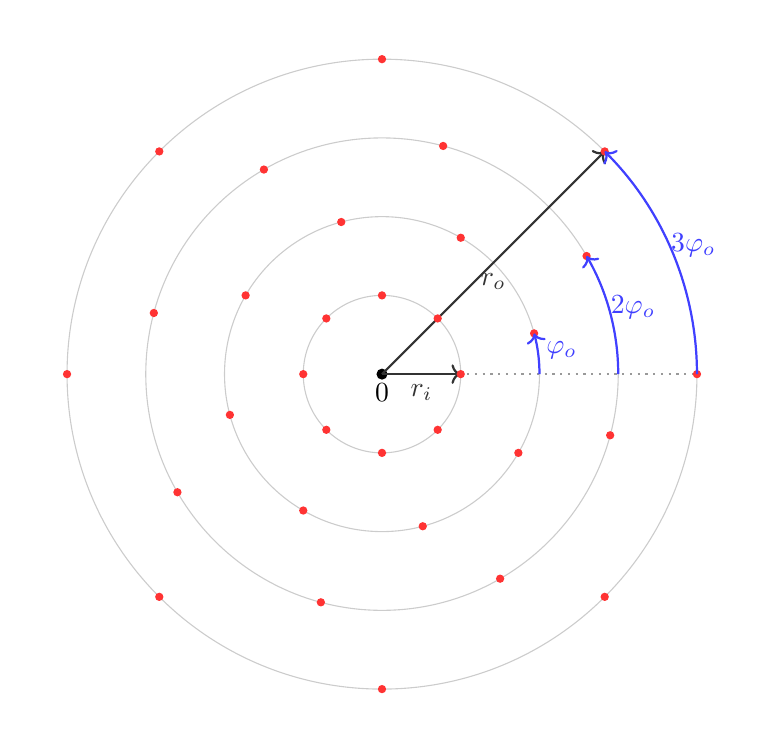
\begin{tikzpicture}
    [
        mymic/.style={circle,fill=red!80, inner sep=0pt,minimum size=3pt},
        lineTh/.style={white!20!black,thick},
        wave/.style={white!80!black,thin},
        wave1/.style={magenta,thick},
        wave11/.style={white!25!blue,thick},
        angle1/.style={white!25!blue,thick},
        wave2/.style={white!60!black,thick}
    ]
%    \draw[style=help lines,step=0.5cm] (-4,-4) grid (4,4);
    \coordinate[label=below:0] (origin) at (0,0);
    \fill[black] (origin) circle (2pt);
    \draw[wave](origin) circle (\ri);
    \draw[wave](origin) circle (\rri);
    \draw[wave](origin) circle (\rrri);
    \draw[wave](origin) circle (\rrrri);
   
    \coordinate[] (r0) at (0:\ri);
    \coordinate[] (r0e) at (4*\ri, 0);
    \coordinate[] (r1) at (15:\rri);
    \coordinate[] (r2) at (30:\rrri);
    \coordinate[] (r3) at (45:\rrrri);
    \coordinate[] (r3r) at (45:\rrrri);
    
    \draw [dotted, wave2] (origin) -- (r0e);
    \draw [->, lineTh] (origin) -- (r0) node[midway,below]{$r_i$};

    % \draw [->, lineTh] (origin) -- (r1) ;
    \draw [->, lineTh] (origin) -- (r3r) node[midway,below]{$r_o$};
    % \draw[wave1, name path=mLine] (w3) -- (w4) ;
    % \draw[wave2, name path=m1line] (origin) -- (m4) ;

    \foreach \i in {0,...,7}
    {
        \node[mymic] at (\i * 360/\b:\ri) {};
        \node[mymic] at (\i * 360/\b + 15:\rri) {};
        \node[mymic] at (\i * 360/\b + 2*15:\rrri) {};
        \node[mymic] at (\i * 360/\b + 3*15:\rrrri) {};
%        \fill[red] (\i * 360/8:3) circle (2pt);  
    }

    
    % \pic [draw,wave1, angle radius=3mm,angle eccentricity=5,pic text=.]
    %     {right angle = w3--origin--w1};
    \pic [draw, ->, wave11,
    angle radius=20mm, angle eccentricity=1.15,"$\varphi_o$"] {angle = r0e--origin--r1};
    \pic [draw, ->, wave11,
    angle radius=30mm, angle eccentricity=1.1,"$2\varphi_o$"] {angle = r0e--origin--r2};
    \pic [draw, ->, wave11,
    angle radius=40mm, angle eccentricity=1.07,"$3\varphi_o$"] {angle = r0e--origin--r3};
    % \pic [draw, ->, wave2,
    % angle radius=25mm, angle eccentricity=1.15,"$\varphi_{m_1}$"] {angle = r0--origin--m4};
    \pgfresetboundingbox
%    \useasboundingbox(-2.6,-2.6)rectangle(2.6,3.6);
    \useasboundingbox(-4.5,-4.4)rectangle(4.5,4.4);
\end{tikzpicture}
\end{document}